% SOURCE: STATE.md Decision Log #5 (deterministic templates, no LLM),
% #6 (mother tier caps at an ACTION, never a number), #7 (the 0.15 top-2
% margin gate; GREEN/AMBER/RED band rule), #8 (LOCAL drivers, not global),
% #11 (band computed once and shared; sign-aware driver ranking, which
% supersedes #8's "top-2 by |SHAP|"), #14 (Hindi authored and clinically
% reviewed by the co-author), #17 (per-tier claim).
% Novelty framed per related_work.md §2 — audience-aware SUPPRESSION, the
% intersection only, mechanism not reclaimed.
% Numbers: results/tables/shap_case_summary.csv (row 66, 0.013/0.487/0.499),
% shap_case_contributions.csv (BS +0.204, BodyTemp +0.094), and the rendered
% artifacts tier_asha_boundary_mid.txt and tier_mother_boundary_mid_hi.txt.
% BUDGET: 2 pp including the figure. If it runs long, cut prose, not the rule.
%
% 2026-09-15 consolidated edit pass (see STATE.md). Four changes:
%   (a) NEW paragraph in 4.2 naming the gate's one-sidedness: the margin test
%       guards the high boundary only, GREEN follows the argmax untested.
%       Framed as unhandled, with the symmetric extension as future work.
%       Paired entry in limitations.tex 6.2. No rule changed in code.
%   (b) NEW 4.4 "When the gate prevents a false alarm", on row 382
%       (0.451/0.097/0.453, true low, predicted high, margin 0.002). Numbers
%       from shap_case_summary.csv. Keeps both honesty sentences: amber on a
%       true-low record is still a false referral; the gate made the error
%       smaller, not correct.
%   (c) The entitlement defence for stripping magnitude MOVED here from
%       related_work.tex 2.4, into the mother-tier paragraph it defends.
%       related_work.tex keeps the literature, the tension and a pointer.
%   (d) 4.5 opener now points to Section 2 for the three literatures instead
%       of restating them with the same cites; figure caption cut to what the
%       figure needs; closing paragraph no longer re-narrates row 66.
\section{Three Tiers from One Prediction}
\label{sec:tiers}

\subsection{What the alarm is, and what derating it means}

By \emph{alarm} we mean the highest-severity signal a tier is permitted to
raise: the red lamp and the urgent spoken message for the mother, the
\textsc{high} header on the health worker's card. The rule this section
describes withholds that signal when the model is close to a coin flip, and
substitutes a middle signal that still says \emph{needs follow-up}.

The direction of that substitution is the whole design, so we state it before
anything else. \textbf{The derate is red to amber, never red to green.} A
near-tie does not mean relax. It means the system is not entitled to the
loudest thing it can say, and falls back to the one below it, which still
sends the mother to a health worker. Nothing here removes a mother from care.

\subsection{The band rule}

Each rendering is driven by one band, computed once per prediction from the
class probabilities and shared across all three tiers:

\begin{itemize}
  \item \textsc{green} if the predicted class is low risk.
  \item \textsc{red} if the predicted class is high risk \emph{and} the
    top-two probability margin is at least $0.15$.
  \item \textsc{amber} otherwise --- which covers every mid-risk prediction
    and every high-risk prediction that sits inside the margin.
\end{itemize}

The threshold of $0.15$ is a design constant. We did not tune it, and no
experiment in this paper supports that value over $0.10$ or $0.20$; we return
to what would be needed to justify it in Section~\ref{sec:limitations}.

The gate is one-sided, and we state where it fires rather than leave a reader
to infer it. The margin test guards the high boundary only: \textsc{green}
follows the argmax with no margin test at all, so a prediction that is
low risk by a hair renders an unqualified all-clear to the mother. That is the
opposite of the asymmetry Section~\ref{sec:data-model} argues for, where
missing a higher-risk mother is the error that matters. The symmetric
extension, derating an ungated near-tie \textsc{green} down to \textsc{amber}
as the red-to-amber move already does, is the natural next version of this
rule and is future work. This version does not implement it.

Computing the band once matters as much as the threshold does. In the first
version of the renderer the health worker's card banded on its own rule and
the mother's lamp banded on this one, so a single prediction could carry two
identities. Section~\ref{sec:eval} describes how that was caught.

\subsection{One prediction, three renderings}

Figure~\ref{fig:tiers} shows the same prediction rendered three ways. The
case is row 66 of the deduplicated set, a true mid-risk record the model
calls high risk, with class probabilities $0.013 / 0.487 / 0.499$ across low,
mid and high. The top-two margin is $0.012$. Blood sugar contributes $+0.204$
to the predicted class and body temperature $+0.094$; the remaining four
features contribute negatively and together amount to less than $0.05$.

\begin{figure}[t!]
\centering
\subcaptionbox{Clinician: signed SHAP contributions, all three class
  probabilities, and the raw readings.\label{fig:tiers-clinician}}%
  {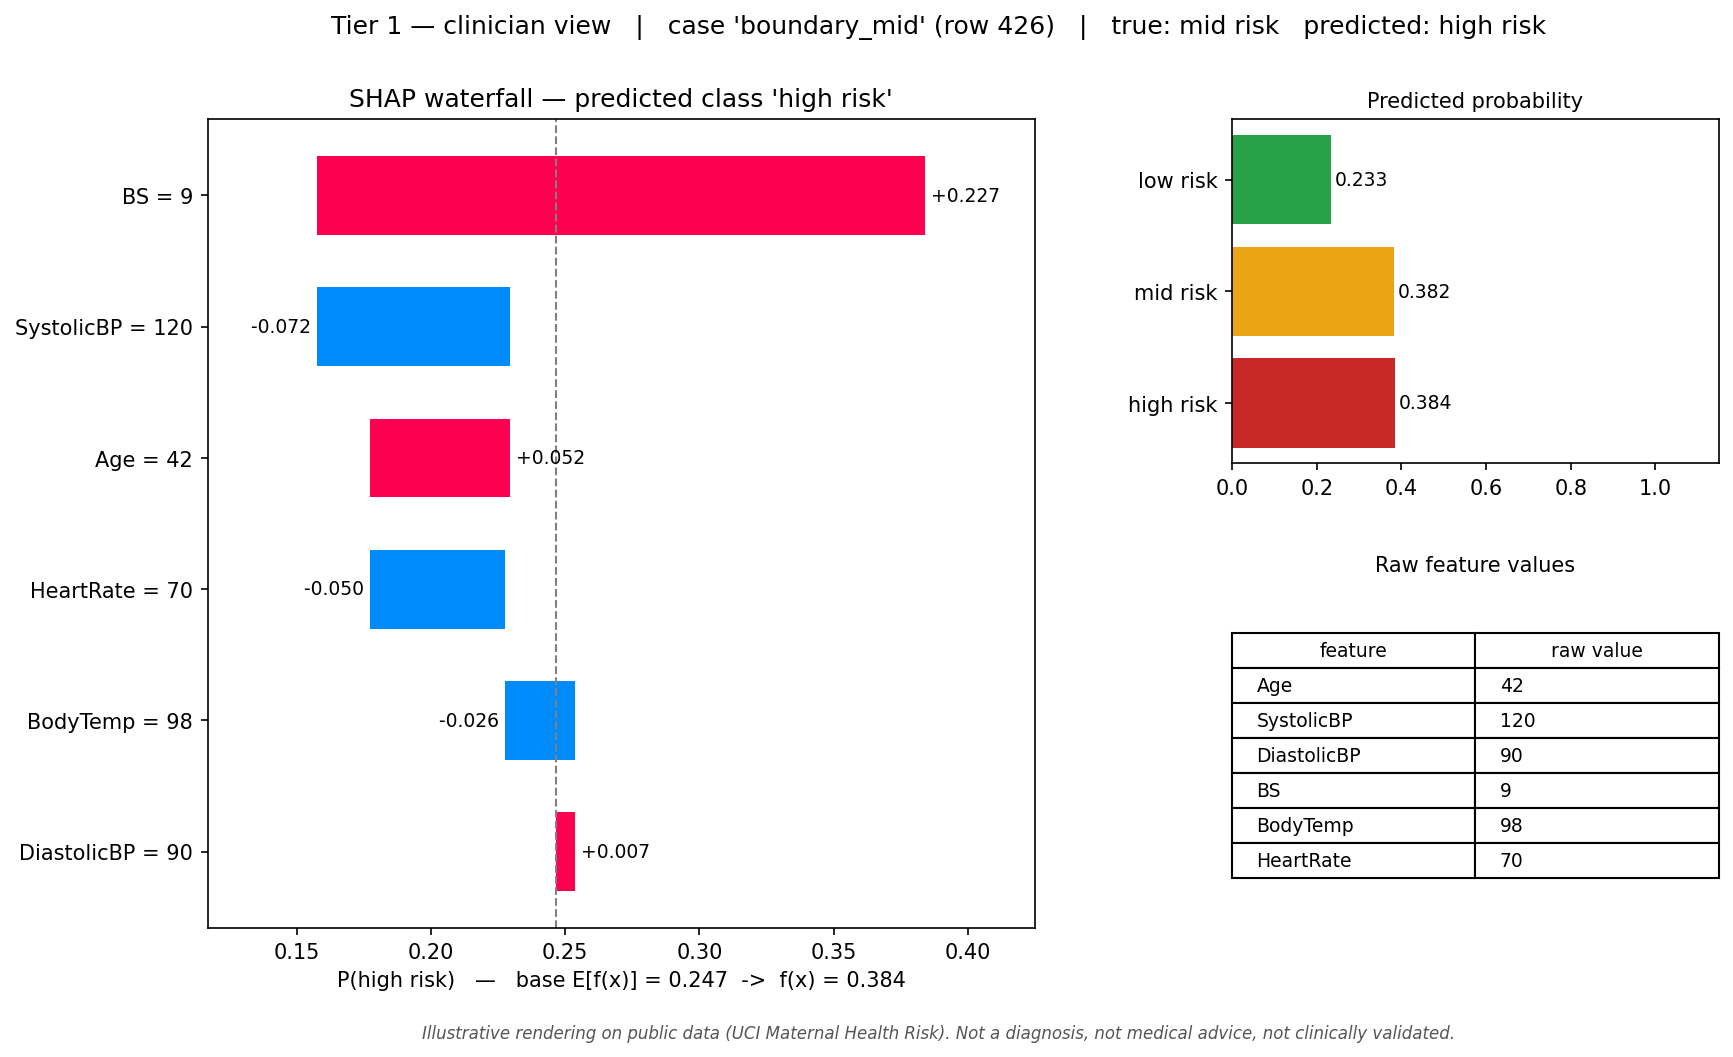
\includegraphics[width=0.94\linewidth]{tier_clinician_boundary_mid.png}}

\vspace{1.2em}

\subcaptionbox{Community health worker: the band header, the two factors
  pushing toward the prediction, and one next step.\label{fig:tiers-asha}}%
  {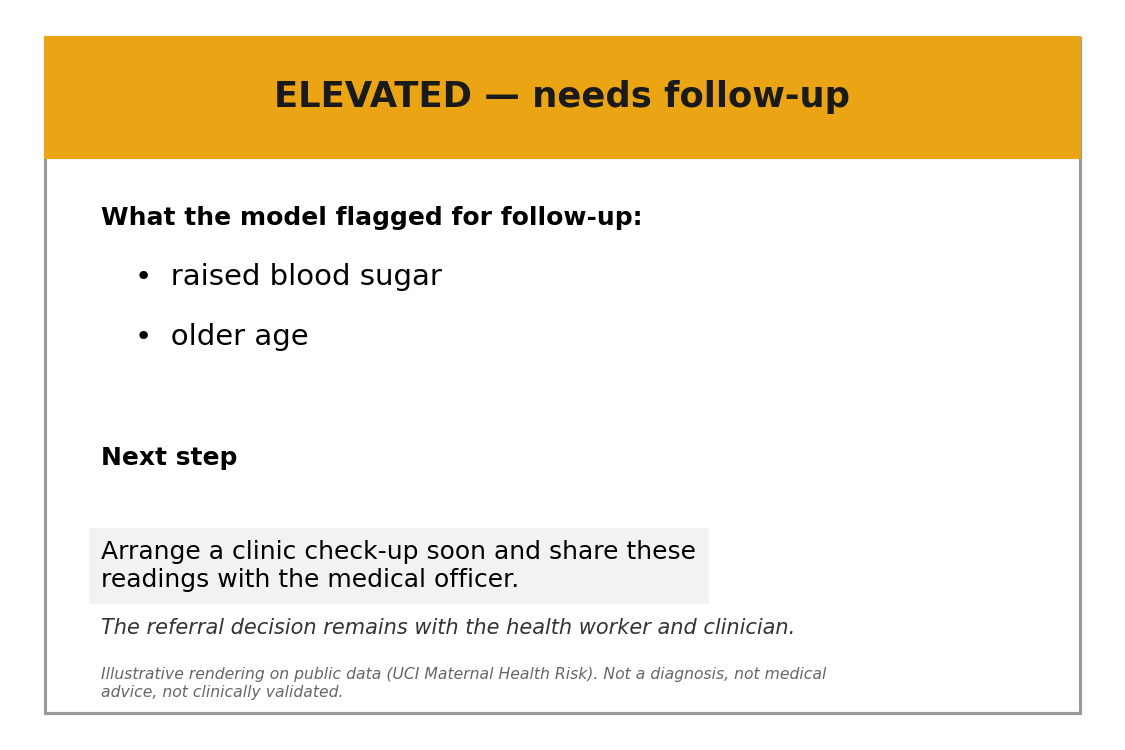
\includegraphics[height=52mm]{tier_asha_boundary_mid.png}}%
\hspace{0.05\linewidth}%
\subcaptionbox{Mother-to-be: amber lit, red
  dark.\label{fig:tiers-mother}}%
  {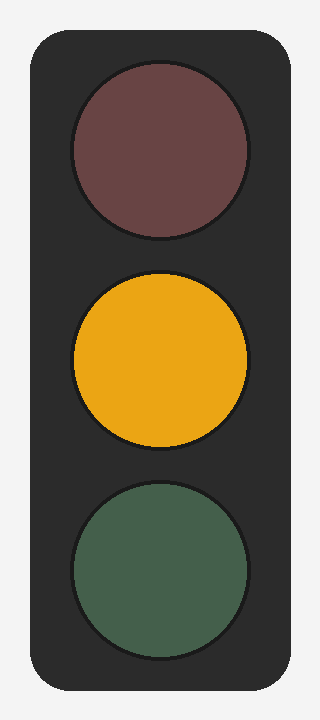
\includegraphics[height=52mm]{tier_mother_boundary_mid.png}}

\caption{Row 66 of the deduplicated set, rendered for all three readers. The
clinician panel carries the near-tie intact at $0.487$ against $0.499$. The
card and the lamp carry the derated band, and the red they would otherwise
have shown is withheld from both. Amber still tells the mother to get checked.
All four cases across all three tiers are in the archived repository.}
\label{fig:tiers}
\end{figure}

\paragraph{Clinician.} The full decomposition, unmodified. Signed SHAP
contributions per feature with numeric labels, all three class probabilities,
and the six raw readings in clinical units. The $0.487$ against $0.499$ is
shown as it stands. A reader who can interrogate the model is given what she
needs to do so, including the fact that the call was nearly a tie.

\paragraph{Community health worker.} A card carrying the band header, the
factors behind \emph{this} prediction, and one next step. Two rules shape it.
The factors are local rather than global: naming the dataset's top features
on every card would print the same two words for every mother and explain
nothing about any of them. And only features that push \emph{toward} the
predicted class are listed, ranked by signed contribution, because a card
headed ``what the model flagged'' that lists a reading arguing against its own
prediction misleads the person making the referral. On this case the card
reads \textsc{elevated --- needs follow-up}, lists raised blood sugar and
raised body temperature, and asks the worker to arrange a check-up and share
the readings. Every string is a fixed template constant filled from the
attributions. No language model runs at inference, which is our stated
alternative to LLM-mediated tiering~\citep{bello2025threelevel}: the card is
regenerable, diffable, and has nothing to hallucinate.

\paragraph{Mother-to-be.} A three-lamp visual and one spoken Hindi sentence.
No probability, no percentage, no condition named, and no text required to
use it. The tier answers \emph{what do I do next}, not \emph{how likely is
this}. Here the amber lamp lights and the message says, in Hindi, that some
findings need attention, not to panic, and to get checked soon at her ANM or
nearest health centre. The Hindi strings were written and clinically reviewed
by the second author, a physician and native speaker; they are neither
machine-translated nor author-invented.

Stripping magnitude departs from the risk-communication literature of
Section~\ref{sec:rw-riskcomm}, which recommends conveying magnitude through an
icon array or a visible denominator, and we take that departure on a stated
condition. An icon array communicates a magnitude the sender is entitled to
assert. At $0.487$ against $0.499$ the model is not so entitled, and rendering
that split as roughly fifty chances in a hundred would carry a precision it
does not have, to the reader least equipped to discount it. Where the
magnitude is trustworthy, show it; where the gate has fired, an ordinal band
and one action is what the model can support. That is the uncertainty argument
of Section~\ref{sec:rw-uncertainty} arriving from the health-communication
side, and it remains an argument rather than a result, since whether the band
is understood as intended is untested here.

\subsection{Derating a false alarm}
\label{sec:tiers-failure}

Row 66 shows the rule behaving correctly on a near-tie between mid and high.
Row 382 shows what it is for. That record is true low risk, the model calls it
high risk at $0.451 / 0.097 / 0.453$ across low, mid and high, and the top-two
margin is $0.002$. A 13-year-old with a body temperature of
101\,\textdegree F, the case Section~\ref{sec:data-age} designates as the
vehicle's failure mode, would have received a red lamp and an urgent spoken
message on the argmax alone. The gate withheld it and both derated channels
show amber instead.

Amber on a true-low record is still a false referral. The gate made the error
smaller, not correct, and it did nothing about the underlying misprediction,
which the clinician tier carries unmodified here as it does on every case.
What it changed is what the mother was told.

\subsection{What we claim}

Section~\ref{sec:related} places the three literatures this design sits in and
states what each has settled: tiering explanations by audience, withholding a
prediction under uncertainty, and fitting a classifier with SHAP attributions
to this dataset. We claim none of them.

What we claim is the intersection, and it is narrow. Prior work on
audience-specific uncertainty makes the \emph{display} of uncertainty
audience-aware~\citep{bhatt2021uncertainty}; the reader with less expertise
receives the same uncertainty in a gentler presentation. Here the abstention
decision is taken once and then rendered as \emph{different assertions}. The
clinician receives $0.487$ against $0.499$. The health worker and the mother
both receive amber, and the red they would otherwise have received is
withheld from each. The gate draws its line at who can interrogate the
model: the reader who can argue with it keeps the split, and the two who
cannot lose the alarm. What separates those two is how much of the model's
state each is asked to hold, not severity. The card carries the drivers and
a next step; the lamp carries neither.

Both cases in this section are ones the model gets wrong. The rendering that
reaches the mother is the one that survives being wrong.
